\section{Graphs}
A \textit{very} common abstract data type, especially in computer science, is the graph. Fundamentally, graphs are used to represent relationships between different objects. Admittedly this is a vague description, but that is because of how incredibly versatile graphs are.

\begin{figure}[h]
    \centering
    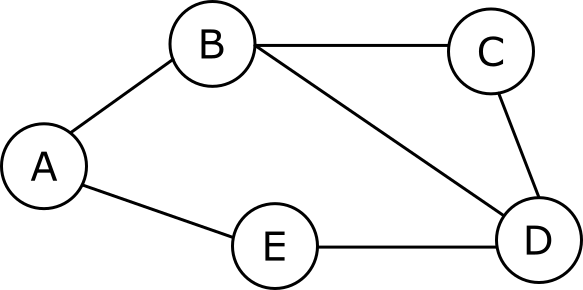
\includegraphics[scale=0.5]{Images/graph_example.png}
    \caption{Example of an undirected graph}
    \label{fig:undir_graph_eg}
\end{figure}

\begin{figure}[h]
    \centering
    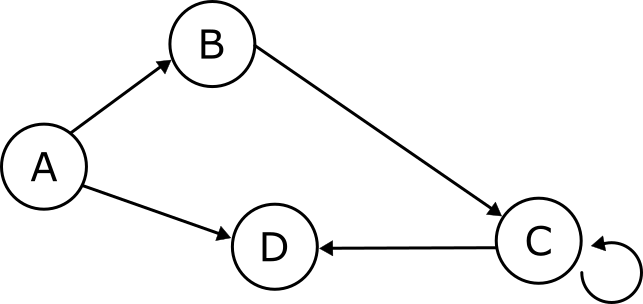
\includegraphics[scale=0.5]{Images/directed_graph_example.png}
    \caption{Example of a directed graph}
    \label{fig:dir_graph_eg}
\end{figure}

Formally, a graph is a tuple $(V, E)$ where $V$ is a set of \textit{vertices} (or nodes) and $E$ is a set of \textit{edges}. A vertex is a single object and an edge is either a tuple of vertices $(v_1, v_2)$ or a 2 element set of vertices $\{v_1, v_2\}$ (we will mostly use the former convention). If a graph is undirected, the order of the vertices in an edge does not matter. That is $(v_1, v_2)$ represents the same edge as $(v_2, v_1)$ (in such cases it may make more sense to use the set notation described previously). In a directed graph $(v_1, v_2)$ and $(v_2, v_1)$ represent different edges. Directed graphs may have self loops, i.e. an edge of the form $(v, v)$ however undirected graphs may not.


If we can `get' from a vertex $u$ to a vertex $v$, then $v$ is said to be adjacent to $u$. To be precise, $v$ is said to be adjacent to $u$ if $(u, v)$ is an edge (if the graph is undirected, then the relationship is symmetric of course: $v$ is adjacent to $u$ if and only if $u$ is adjacent to $v$. However this is not the case with directed graphs).

For undirected graphs, we say the edge $(u, v)$ is incident on vertices $u$ and $v$. If this was a directed graph instead, we would say the edge $(u, v)$ is incident \textit{from} $u$ and is incident \textit{to} $v$.

An important quantity is the degree of a vertex, which is roughly a measure of how connected the vertex is. For undirected graphs, this is simply the number of edges of incident on a vertex. As usual, we need to differentiate between the two types of edges we may have for any vertex in a directed graph. So we have the in-degree which is the number of edges incident to $v$ (i.e. the number of edges going into $v$) and the out-degree which is the number of edges incident from $v$ (i.e. the number of edges leaving $v$). 

A natural attribute to consider now is the neighbourhood of a vertex, which would be the vertices you can immediately get to or from a given vertex. For directed graphs, we have in-neighbourhoods where the in neighbourhood of $v$, is the set of vertices $u$ where $(u, v)$ is an edge (these are all vertices that can get to $v$ in `one step'.) and the out-neighbourhood which is the set of vertices $w$ such that $(v, w)$ is an edge (these are all the vertices that $v$ can reach in `one step'). If the graph is undirected then the two sets are the same and we simply call it the neighbourhood of $v$. 

Finally sometimes we wish to associate real numbers to each of the edges to get a weighted graph. The associated real number for each edge is called the edge cost or edge weight.

Immediately when one sees a graph, one is tempted to talk about paths which is exactly what one would expect. Formally, a path is a list of edges of the form $(v, u_1), (u_1, u_2), \dots, (u_{k - 1}, x)$ (perhaps you might have expected a path to be a list of vertices where there exists an edge between every consecutive part of vertices. The two definitions are obviously equivalent and which one we choose is largely a matter of taste). We will define the length of a path to be the number of edges on the path. A cycle is a path (with no repeating edges) that begins and ends with the same vertex. A simple cycle is one where the only vertex that repeats is the first (and last) one. A graph is said to be acyclic if it has no cycles.

A graph is said to be connected if there is a path between every pair of vertices. For disconnected graphs, we often talks about its connected components, which are again what you would expect (we don't need a precise definition here, but the formal definition involves defining two vertices to be equivalent if there exists a path between them and then the connected components are simply the equivalence classes).

At this point the reader may realize that we have already worked with some special graphs a lot, namely trees! To be precise, a tree is simply an undirected, connected, acyclic graph (in fact this is a definition). If we have a special vertex, which we call a root, we get a rooted tree. Non-rooted trees are sometimes called free trees. Finally a disjoint union of trees is (delightfully) called a forest. In other words, a forest is a graph where every connected component is a tree.

Thus graphs are generalizations of trees. Given how useful trees have been, one can only imagine how useful graphs will be!

\begin{remark}
    Whether or not two graphs are the same is entirely dependent on the connections and vertices of the graphs, not on how we draw them. Although this might seem obvious, it is often easy to forget since there are many ways we might draw a particular graph and it's not always obvious whether two graphs really are the same or different.
\end{remark}

\begin{figure}[h]
    \centering
    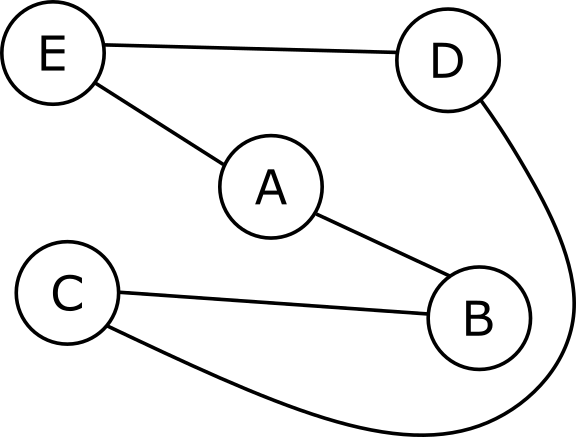
\includegraphics[scale=0.5]{Images/equiv_graph.png}
    \caption{An equivalent graph to \autoref{fig:undir_graph_eg}}
    \label{fig:equiv-graph}
\end{figure}

\subsection{Graph Representations}

There are two common ways of representing graphs: adjacency lists and adjacency matrices. An adjacency list is a list (most likely in an array) of all the vertices in the graph where each vertex points to a linked list of its (out) neighbours. For an adjacency matrix, on the the other hand, we simply say whether or not a given edge is present and present this information in matrix form where 1 represents the existence of a matrix and 0 its non-existence. 

If the graph is undirected then the matrix will be symmetric with 0s down the diagonal. This need not be the case directed graphs. Additionally for directed graphs, we need to decide whether a 1 in row $i$ and column $j$ represents the edge $(i, j)$ or $(j, i)$. We will use the former convention (recall that the element in row $i$ and column $j$ is in the $(i, j)$ spot. This makes it easier to remember the convention). In other words, the matrix entries $a_{ij}$ are given by
$$ a_{ij} = \begin{cases}
1 &\text{ if } (i, j) \in E\\
0 &\text{ otherwise}
\end{cases}
$$
As an example, the adjacency matrix for the undirected graph in \autoref{fig:undir_graph_eg} is
\begin{align*}
    \begin{pmatrix}
    0 & 1 & 0 & 0 & 1\\
    1 & 0 & 1 & 1 & 0\\
    0 & 1 & 0 & 1 & 0\\
    0 & 1 & 1 & 0 & 1\\
    1 & 0 & 0 & 1 & 0
    \end{pmatrix}
\end{align*}
and the matrix for the directed graph in \autoref{fig:dir_graph_eg} is
\begin{align*}
    \begin{pmatrix}
        0 & 1 & 0 & 1\\
        0 & 0 & 1 & 0\\
        0 & 0 & 1 & 1\\
        0 & 0 & 0 & 0
    \end{pmatrix}
\end{align*}

It is clear that the spatial complexity of adjacency matrices is $O(|V|^2)$ (recall that $|S|$ for a set $S$ is the number of elements in $S$ or its cardinality). With a bit of thinking we realise that the spatial complexity of adjacency lists is larger of $|V|$ and $|E|$ (you might think that the complexity should be $|E|$ but we always need an array of size $|V|$ to have every vertex point to its neighbourhood even if the neighbourhood is empty). Thus we can say that the spatial complexity of adjacency lists if $O(|V| + |E|)$.

Now let us consider the time complexity of these representations. The basic operations of graphs are adding/removing vertices, adding/removing edges, verifying if an edge is present (known as edge query) and finding the neighbourhood of a vertex (where finding the in-neighbourhood and out-neighbourhood are two separate operations if $G$ is directed). In most cases, the complexity will depend on how we are implementing the representations. For example, if we are storing the matrix in an array then adding new vertices would require us to copy elements into a new array making the operation $O(|V|^2)$ in this case. On the other hand if adjacency lists are stored as an array of (pointers to) linked lists then adding a new vertex is constant (we add an empty linked list to the end of this array).

\subsection{Breadth First Search}
One of the most common things we want to do is walk through a graph while perhaps applying some operation on each vertex. Breadth-first search is one such method for walking through a graph. If one thinks of the special case of the tree, the strategy (and name) are easier to understand. The idea is we search broadly first before diving deep (i.e. we explore all the vertices at a particular depth before exploring their children). The counterpart is of course to dive deep before searching broadly, known reasonably enough as Depth First Search, will be discussed later. 

By starting a vertex $s$ (short for \textit{source}), we find paths from $s$ to reachable vertices $v$. We can use these paths to construct a tree rooted at $s$. This is called the BFS tree. 

A thing we very often do with graphs is colour the vertices. This means we classify the vertices into certain categories. We will see this technique in the BFS algorithm. In particular, we will have 3 colours: white, grey and black. White vertices will be ones we haven't discovered yet. Grey vertices are vertices which have been discovered but not fully explored (it may have edges we haven't gone down). Finally black vertices have been explored fully. In addition, to the colour of each vertex, we will also keep track of the parent of each vertex and its distance from $s$.

\begin{figure}[h]
    \centering
    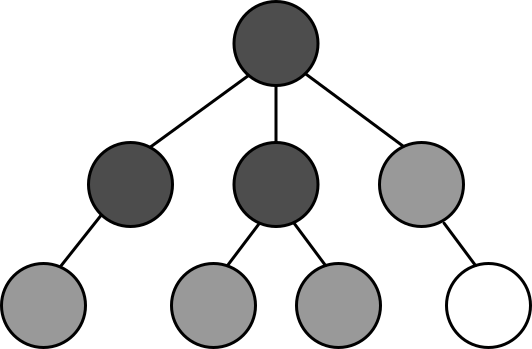
\includegraphics[scale=0.4]{Images/bfs_search.png}
    \caption{Example of vertex colouring for BFS}
    \label{fig:bfs-example}
\end{figure}

\begin{lstlisting}
BFS(G = (V, E), s):
    # we first initialise the graph with appropriate values
    for v in V:
        colour[v] = white
        d[v] = inf # distance from s/depth of node in BFS tree
        p[v] = null # parent, pi is another commonly used symbol
    
    # initialising s
    colour[s] = grey
    d[s] = 0
    initialise empty queue Q # Q will store the grey vertices, handled in FIFO order
    ENQUEUE(Q, s)
    
    while Q is not empty:
        u = DEQUEUE(Q, s)
        for each edge (u, v) in E:
            if colour[v] == white:
                colour[v] = grey
                d[v] = d[u] + 1
                p[v] = u
                ENQUEUE(Q, v)
        colour[u] = black
\end{lstlisting}

Let us consider the complexity of this algorithm. First we see that each node is enqueued at most once (namely if it is connected to $s$ or reachable from $s$). So the while loop iterates at most $|V|$ times. Moreover the while and for loop combined iterate over all the edges in $G$. Therefore the run time of this algorithm is $O(|V| + |E|)$ (if $|E| < |V|$ then we might still need to iterate over all the vertices so we again have the case that the runtime is bounded by the larger of the two).\\

We claim that the BFS satisfies a very neat property: namely the $d[u]$ of each vertex after the algorithm is shortest distance from $s$ to the vertex $u$. By definition this is the smallest number of edges on any path from $s$ to $u$ (this definition will alter slightly when we consider weighted graphs). 

Let $\delta(s, v)$ denote the shortest distance between $s$ and $v$. First we claim that $\delta(s, v) \leq \delta(u, v) + 1$ for all $(u, v) \in E$. This is obvious if $v$ is not reachable from $s$ (this means that if $(u, v) \in E$ then $u$ is not reachable from $s$ so the right hand side is $\infty$). Suppose $v$ is reachable from $s$ then. Suppose $p$ is a path from $s$ to $v$. If we remove the last edge from $p$, we get a path from $s$ to some $u$. By definition, the length of this path must be greater than or equal to $\delta(s, u)$ (remember that $\delta(s, u)$ is the length of the shortest path so all other paths must be bigger or equal in length). Then the length of $p$ is at least $\delta(s, u) + 1$. Once again we use the definition of $\delta$ to conclude that $\delta(s, v) \leq \delta(s, u) + 1$.

Next we claim that $d[v] \geq \delta(s, v)$ for all $v \in V$ at any point during BFS. Clearly this holds at the beginning (line 14) as $d[s] = 0 = \delta(s, s)$ and $d[v] = \infty$ for all other $v$. We inductively assume the claim holds for some sequence of \ttt{ENQUEUE} and \ttt{DEQUEUE} operations and we will show it holds immediate after one of these operations as well. Suppose we enqueue a vertex $v$. Then we must have discovered it from a vertex $u$ which was queued before. Therefore $d[u] \geq \delta(s, u)$. Additionally by line 19 of the algorithm, we know that $d[v] = d[u] + 1$, allowing us conclude that $d[v] \geq \delta(s, u) + 1$ which we know to be greater than or equal to $\delta(s, v)$ by the previous lemma. Since we never change $d[v]$ again, the claim holds.

The next lemma is that if $Q = [v_1, \dots, v_r]$ then $d[v_i] \leq d[v_{i + 1}]$ and moreover that $d[v_r] \leq d[v_1] + 1$. This mean that the distances in the queue at any time are non-decreasing and can differ by at most 1. We will induct similarly to before. Clearly this holds in the base case when $Q = [s]$ (there is only one element!). So suppose the statement holds when $Q = [v_1, \dots, v_r]$ and we will show it holds whenever we \ttt{ENQUEUE} or \ttt{DEQUEUE} from this point. Dequeuing is the easier one to consider. Since we are assuming $Q$ to be non-decreasing to be begin with, removing $v_1$ doesn't change this and $v_2$ is made the new first element (or $Q$ is empty now which is also fine). Since $v_1 \leq v_2$ and $v_r \leq v_1 + 1$, we must have that $v_r \leq v_2 + 1$ preserving the second property. Now suppose we enqueue a vertex $v$, making it now $v_{r+1}$. By looking at the code, we see that this occurs after dequeuing its parent $u$. Then $d[v] = d[u] + 1$. By assumption $d[u] \leq d[v_1]$ therefore $d[v] = d[v_{r + 1}] \leq d[v_1] + 1$. By assumption we know that $d[v_r] \leq d[v_1] + 1$ so the non-decreasing property is maintained as well.

\begin{theorem}
After we run BFS(G, s), $d[v] = \delta(s, v)$ for every $v \in V$.
\end{theorem}
\begin{proof}
We prove this using contradiction. Let $v$ be a vertex where $d[v] > \delta(s, v)$ for the minimum such $\delta(s, v)$ (we already know that $d[v]$ cannot be less than $\delta(s, v)$ by the first claim shown above). This means that for all $u$ where $\delta(s, u) < \delta(s, v)$ then $d[u] = \delta(s, u)$. Let $u$ be $v$'s preceding vertex in the minimal path from $s$ to $v$. Then we know that $d[u] = \delta(s, u)$ (indeed it is not hard to see that $\delta(s, u) = \delta(s, v) - 1$). Thus our assumption is equivalent to $d[v] > d[u] + 1$.

Now suppose we have dequeued vertex $u$ and are exploring the edge $(u, v)$. There are three possible colourings that $v$ could have. If $v$ is white then $d[v]$ is set to $d[u] + 1$ (and never reset to anything else), leading to a contradiction. If $v$ is black, then it appeared in the queue before $u$ so $d[v] \leq d[u]$ (remember we have non-decreasing distances in $Q$). This leads us to another contradiction. The final possibility is that $v$ is grey. This means $v$ is currently in $Q$ (this is where all the grey vertices are stored). Then before $u$ was dequeued, $u$ and $v$ were simultaneously in $Q$. We know then that $d[v] \leq d[u] + 1$ (distances in the queue can differ by at most 1) giving us our final contradiction.
\end{proof}